\chapter{ Аналитический раздел}
\label{cha:analysis}

% Выбрали для распараллеливания трассировку. !!! Ok.

% В рисунках не нужны точки в конце подписи. Ok.
% Схема алгоритма главного потока (исправить подписи к листингу) ? На что...?

% Список литературы
% НАЗВАНИЕ [эл ресурс]. Режим доступа: ССЫЛКА (дата обращения: ДАТА).
% Добавить в литру с#

% "МЫ" УБРАТЬ. Ok.

% Убрать точку в подписях листингах.OK.

Для данной лабораторной работе, которая предполагает распараллеливание 
знакомого нам алгоритма был выбран алгоритм трассировки лучей. 
В данной части будет рассмотрено теоретическое описание алгоритмов.

\section{Алгоритм прямой трассировки лучей}

Для понимания алгоритма обратной трассировки лучей следует изначально разобраться с
алгоритм прямой трассировки лучей.

Основная идея алгоритма прямой трассировки лучей состоит в том, что на­блюдатель 
видит объекты, благодаря световым лучам, испускаемым некоторым ис­точником,
которые падают на объект, отражаются, преломляются или проходят че­рез
него и в результате достигают нас. Если проследить за лучами, то становится
понятно, что среди них лишь малая часть дойдет до наблюдателя, что приведет к
большим затратам ЭВМ. Заменой данному алгоритму служит метод обратный трас­сировки лучшей.

\section{Алгоритм обратной трассировки лучей}

Алгоритм обратной трассировки лучей отслеживает лучи в обратном направ­ление (от наблюдателя к объекту).
Считается, что наблюдатель расположен на положительной полуоси z в бес­конечности,
поэтому все световые лучи параллельны оси z. В ходе работы испуска­ются
лучи от наблюдателя и ищутся пересечения луча и всех объектов сцены.
В результате пересечение с максимальным значением z является видимой частью
поверхности и атрибуты данного объекта используются для определения характери­стик
пикселя, через центр которого проходит данный световой луч. Эффективность
процедуры определения пересечений луча с поверхностью объекта оказывает самое
большое влияние на эффективность всего алгоритма. Чтобы избавиться от ненуж­ного
поиска пересечений было придумано искать пересечение луча с объемной обо­лочкой
рассматриваемого объекта. Под оболочкой понимается некоторый простой
объект, внутрь которого можно поместить рассматриваемый объект, к примеру па­раллелепипед или сфера (рис. \ref{ref:img}).

\begin{figure}[ht!]
	\centering{
		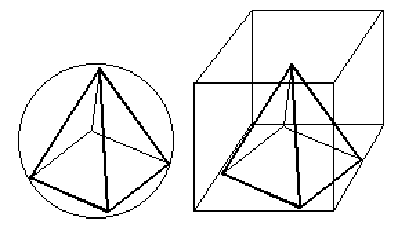
\includegraphics[width=0.6\textwidth]{img/shell.png}
		\caption{Сферическая и прямоугольная оболочки}
		\label{ref:img}}
\end{figure}

В дальнейшем при рассмотрении пересечения луча и объемной оболочкой
рассматриваемого объекта, если такого пересечения нет, то и соответственно пере­сечения
луча и самого рассматриваемого объекта нет, и наоборот, если будет найдено
пересечение, то возможно, есть пересечение луча и рассматриваемого объекта. Для
расчета эффектов освещения сцены проводятся вторичные лучи от точек пересече­ния
ко всем источникам света. Если на пути этих лучей встречается непрозрачное
тело, значит данная точка находится в тени, иначе он влияет на освещение данной
точки. Также для получения более реалистичного изображения сцены, нужно учи­тывать
вклады отраженных и преломленных лучей.
К недостатку алгоритма относится его производительность.

\section{Применение алгоритма}

Алгоритм трассировки лучей используется для визуализации
реалистического изображения, учитывая тени, отражение объектов, преломление и т.д.
Данный алгоритм активно используется, к примеру, в игровой индустрии.

\section{Параллельная реализация алгоритма обратной трассировки лучей}

Поскольку алгоритм обратной трассировки лучей обрабатывает каждый пиксель
экрана независимо, можно распараллелить обработку всего экрана, разбив
его на некоторые части. В данной лабораторной работе будет представлено 
разбиение горизонтально и вертикально. Т.е. каждый поток будет обрабатывать
свой участок экрана. 

На рис. \ref{ref:img1} показано, как можно вертикально разбить экран на 
несколько частей. На рис. \ref{ref:img2} показано горизонтальное разбиение экрана.
Разбив экран на части можно реализовывать параллельное вычисление цвета 
пикселей каждой части экрана.

\begin{figure}[ht!]
	\centering{
		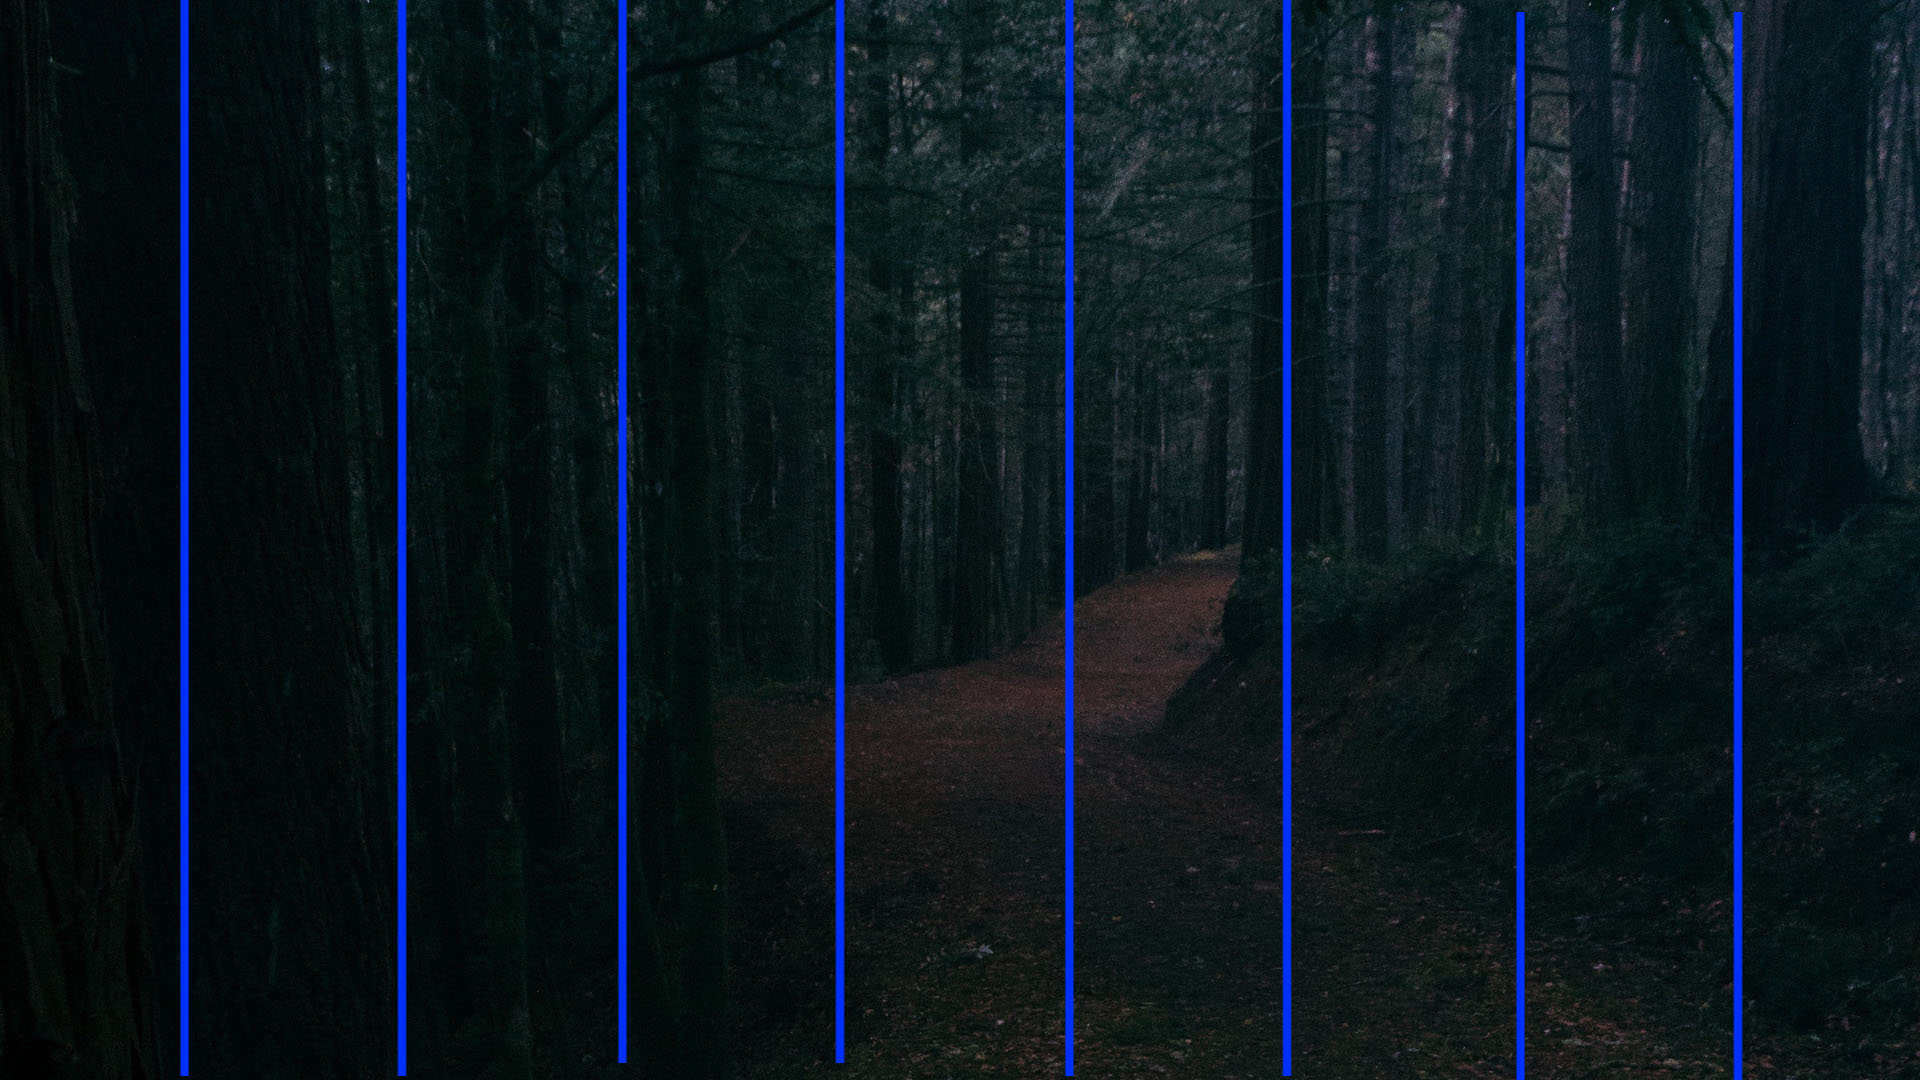
\includegraphics[width=0.8\textwidth]{img/h.jpg}
		\caption{Вертикальное разбиение экрана}
		\label{ref:img1}}
\end{figure}

\begin{figure}[ht!]
	\centering{
		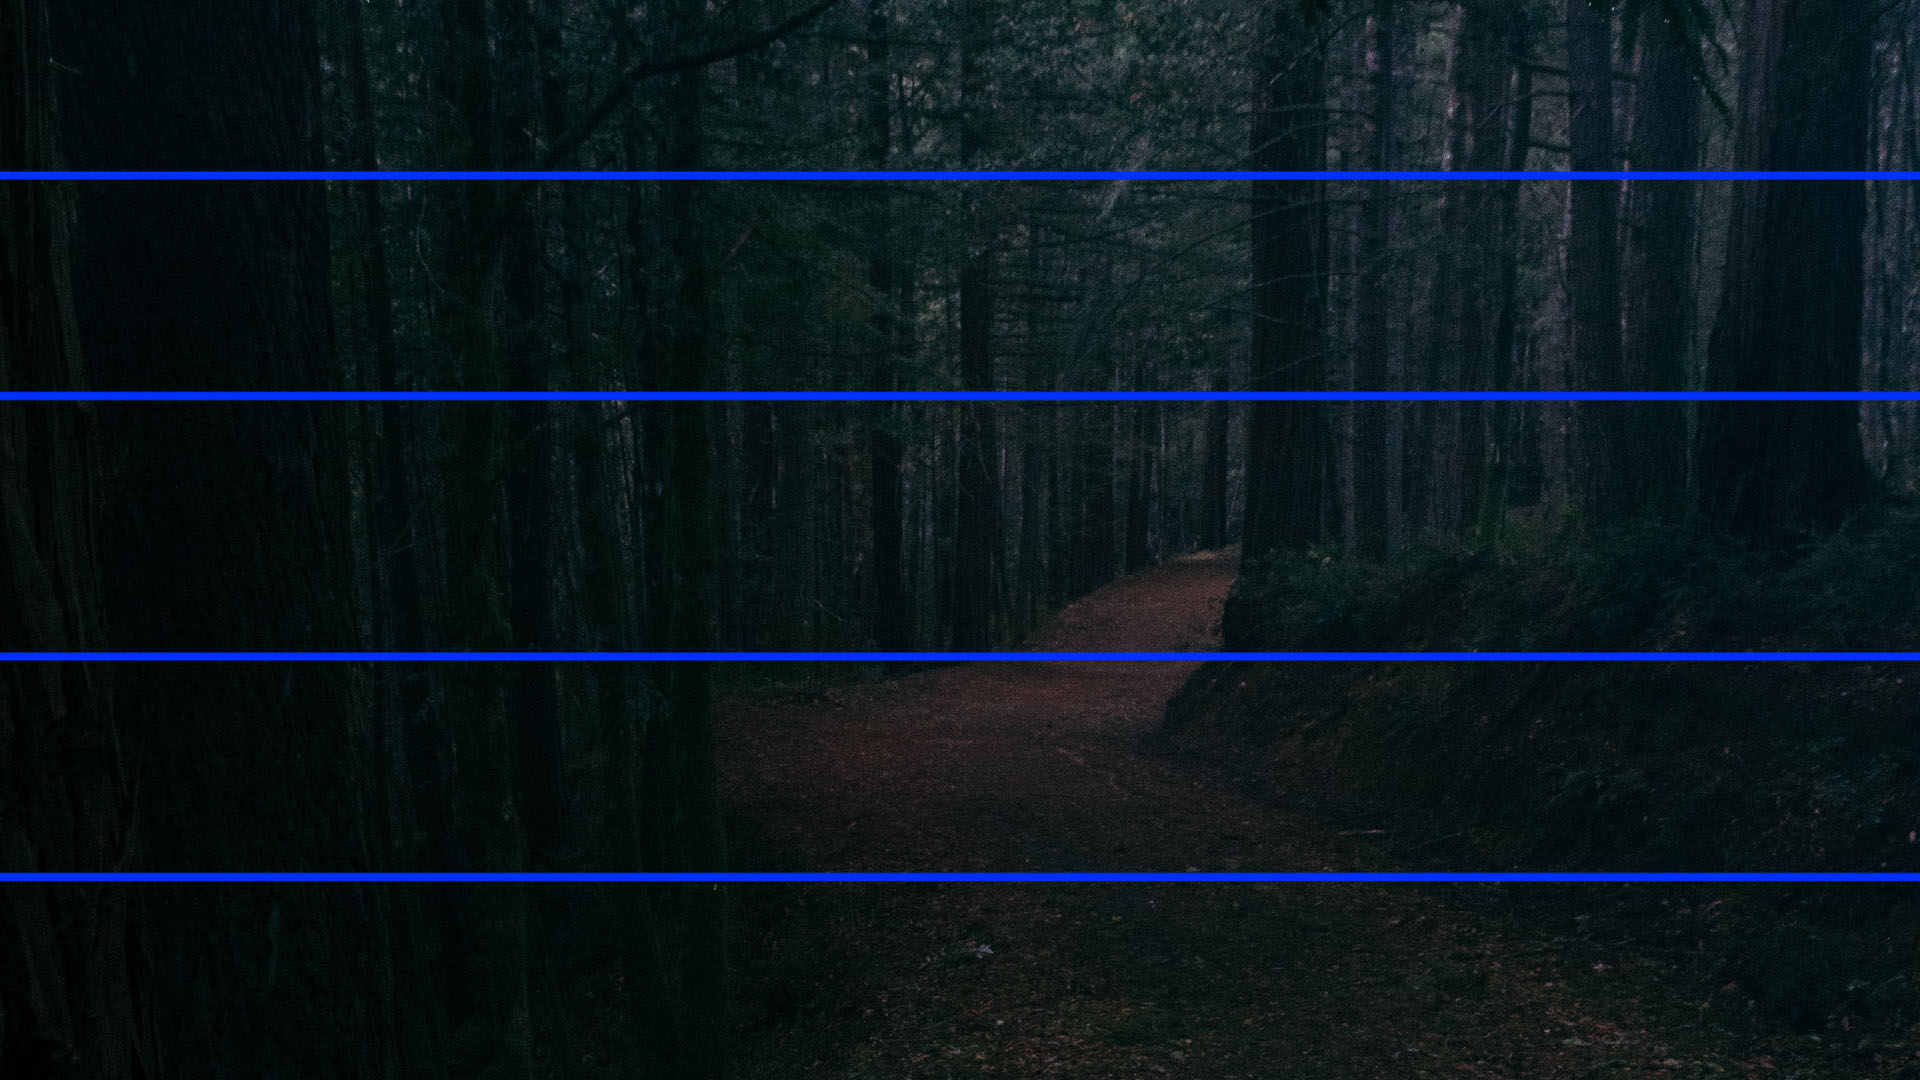
\includegraphics[width=0.8\textwidth]{img/w.jpg}
		\caption{Горизонтальное разбиение экрана}
		\label{ref:img2}}
\end{figure}

\section{Вывод}

В данном разделе были рассмотрены
основополагающие материалы, которые в дальнейшем потребуются
при параллельной и однопоточной реализации алгоритма трассировки лучей.  
